\documentclass[12pt]{article}
\usepackage{graphicx} % Required for inserting images
\usepackage{enumitem}
\usepackage{mathtools}
\usepackage{amsmath}
\usepackage{gvv-book}
\usepackage{gvv}

\title{\textbf{5.2.7}}
\author{\textbf{EE25BTECH11004 - Aditya Appana}}
\date{September 20, 2025}

\begin{document}

\maketitle

\section*{Question}
Solve the following system of linear equations.\\
$$\frac{3}{2}x + \frac{5}{3}y= 7$$
$$9x-10y=14$$

\section*{Solution}

Organizing the given equations into an augmented matrix:
\begin{align}
\myvec{\frac{3}{2}& \frac{5}{3} & 7 \\ 9 & -10 & 14}
\end{align}\\
Performing row operations:
\begin{align}
\myvec{\frac{3}{2}& \frac{5}{3} & 7 \\ 9 & -10 & 14} \xrightarrow{\text{R_2 \rightarrow $R_2- 6R_1$}}
 \myvec{\frac{3}{2}& \frac{5}{3} & 7 \\ 0 & -20 & -28}  \xrightarrow{\text{R_1 \rightarrow $R_1+ \frac{1}{12}R_2$}} \myvec{\frac{3}{2}& 0 & \frac{14}{3} \\ 0 & -20 & -28} 
\end{align}\\
Solving, we get the solution as:
\begin{align}
\vec{x}= \myvec{\frac{28}{9}\\\frac{7}{5}}
\end{align}

\begin{figure}[H]
    \centering
    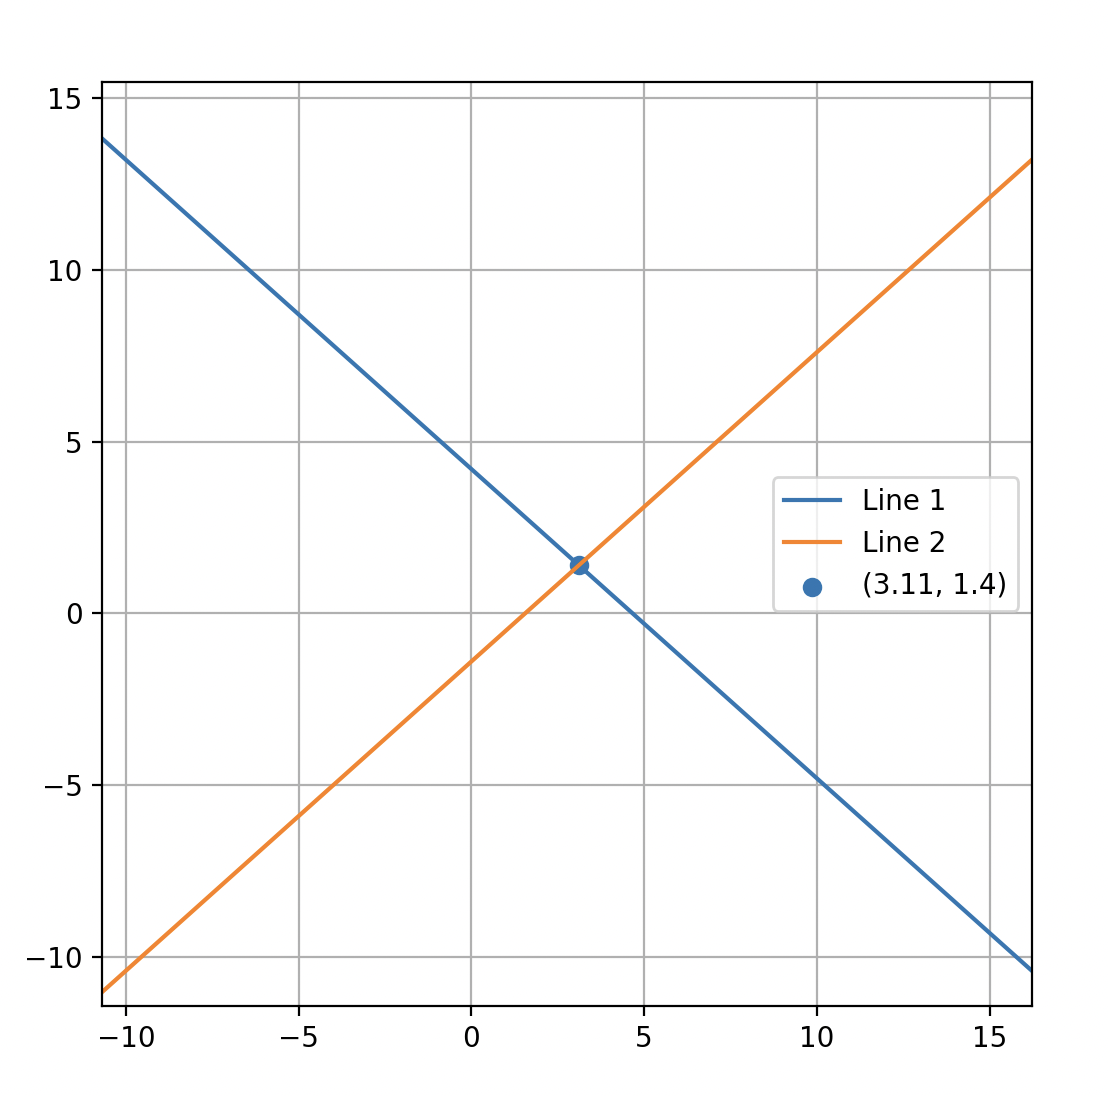
\includegraphics[width=0.9\columnwidth]{Figs/527.png}
    \caption{Plot}
    \label{fig:placeholder}
\end{figure}

\end{document}